%\documentclass[aspectratio=169]{beamer}
\documentclass{beamer}

\usetheme{Singapore}
\setbeamercolor{alerted text}{fg=orange}
\setbeamercolor{background canvas}{bg=black}
\setbeamercolor{block body alerted}{bg=normal text.bg!90!black}
\setbeamercolor{block body}{bg=normal text.bg!90!black}
\setbeamercolor{block body example}{bg=normal text.bg!90!black}
\setbeamercolor{block title alerted}{use={normal text,alerted
text},fg=alerted text.fg!75!normal text.fg,bg=normal text.bg!75!black}
\setbeamercolor{block title}{bg=blue}
\setbeamercolor{block title example}{use={normal text,example
text},fg=example text.fg!75!normal text.fg,bg=normal text.bg!75!black}
\setbeamercolor{fine separation line}{}
\setbeamercolor{frametitle}{fg=white}
\setbeamercolor{item projected}{fg=black}
\setbeamercolor{normal text}{bg=black,fg=white}
\setbeamercolor{palette sidebar primary}{use=normal text,fg=normal
text.fg}
\setbeamercolor{palette sidebar
quaternary}{use=structure,fg=structure.fg}
\setbeamercolor{palette sidebar
secondary}{use=structure,fg=structure.fg}
\setbeamercolor{palette sidebar tertiary}{use=normal text,fg=normal
text.fg}
\setbeamercolor{section in sidebar}{fg=brown}
\setbeamercolor{section in sidebar shaded}{fg=grey}
\setbeamercolor{separation line}{}
\setbeamercolor{sidebar}{bg=red}
\setbeamercolor{sidebar}{parent=palette primary}
\setbeamercolor{structure}{bg=black, fg=black}
\setbeamercolor{subsection in sidebar}{fg=brown}
\setbeamercolor{subsection in sidebar shaded}{fg=grey}
\setbeamercolor{title}{fg=white}
\setbeamercolor{titlelike}{fg=white}

\title{Memory Efficiency and Conflict-free Replicated Data Types}
\author{Ryan Bruno \and Dr. Armstrong}
\date{October 30, 2020}

\begin{document}
    % Title Frame
    \begin{frame}
        \titlepage
    \end{frame}
    \begin{frame}[shrink]
        \frametitle{Problem Description}
        \begin{center}
        \begin{minipage}{4in}
          Conflict-Free Replicated Data Types (CRDTs) use extra metadata
          to allow for concurrent modifications of data without
          consensus. How can we reduce the this overhead?
        \end{minipage}
        \end{center}
    \end{frame}
    \begin{frame}[shrink]
        \frametitle{CRDT Background Information}

        \textbf{Applies to Distributed Systems with Eventual Consistency.}

        Provides Guarantees:

        \begin{enumerate}
        \item - Merge consistently.
        \item - No writes (or modifications) can be lost.
        \end{enumerate}

        OR-Set

    \end{frame}
    \begin{frame}
        \frametitle{What is Eventual Consistency?}

        CAP Theorem = Consistency, Availability, network Partitioned

        \begin{center}
        \begin{minipage}{4in}
         During a network Partition between nodes a system cannot be
         both {\color{red}Consistent} and {\color{green}Available}.
        \end{minipage}
        \end{center}
        \begin{center}
        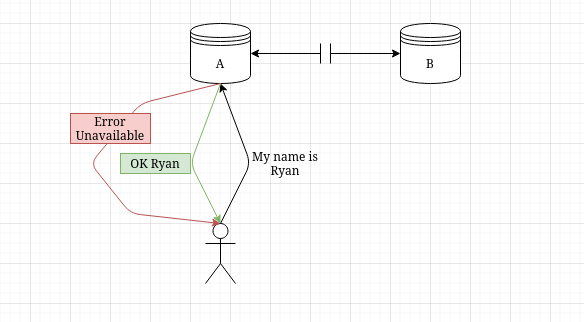
\includegraphics[width=.75\textwidth]{CapDiagram}
        \end{center}
    \end{frame}

    \begin{frame}[shrink]
        \frametitle{CRDT Background Information}

        Applies to Distributed Systems with Eventual Consistency.

        \textbf{Provides Guarantees:}

        \begin{enumerate}
            \item \textbf{- Merge consistently.}
            \item \textbf{- No writes (or modifications) can be lost.}
        \end{enumerate}

        \textbf{OR-Set}

    \end{frame}

    % CRDT
    \begin{frame}
        \includegraphics[page=1,width=\textwidth]{original}
    \end{frame}
    \begin{frame}
        \includegraphics[page=2,width=\textwidth]{original}
    \end{frame}
    \begin{frame}
        \includegraphics[page=3,width=\textwidth]{original}
    \end{frame}
    \begin{frame}
        \includegraphics[page=4,width=\textwidth]{original}
    \end{frame}
    \begin{frame}
        \includegraphics[page=5,width=\textwidth]{original}
    \end{frame}
    \begin{frame}
        \includegraphics[page=6,width=\textwidth]{original}
    \end{frame}
    \begin{frame}
        \includegraphics[page=7,width=\textwidth]{original}
    \end{frame}
    \begin{frame}
        \includegraphics[page=8,width=\textwidth]{original}
    \end{frame}
    \begin{frame}
        \includegraphics[page=9,width=\textwidth]{original}
    \end{frame}
    \begin{frame}
        \includegraphics[page=10,width=\textwidth]{original}
    \end{frame}

    \begin{frame}
        \begin{center}
            \large{We have a problem:}
            \pause

            \large{Unbounded growth of tombstones.}
        \end{center}
    \end{frame}

    \begin{frame}[shrink]
        \frametitle{What does unbounded growth look like?}
        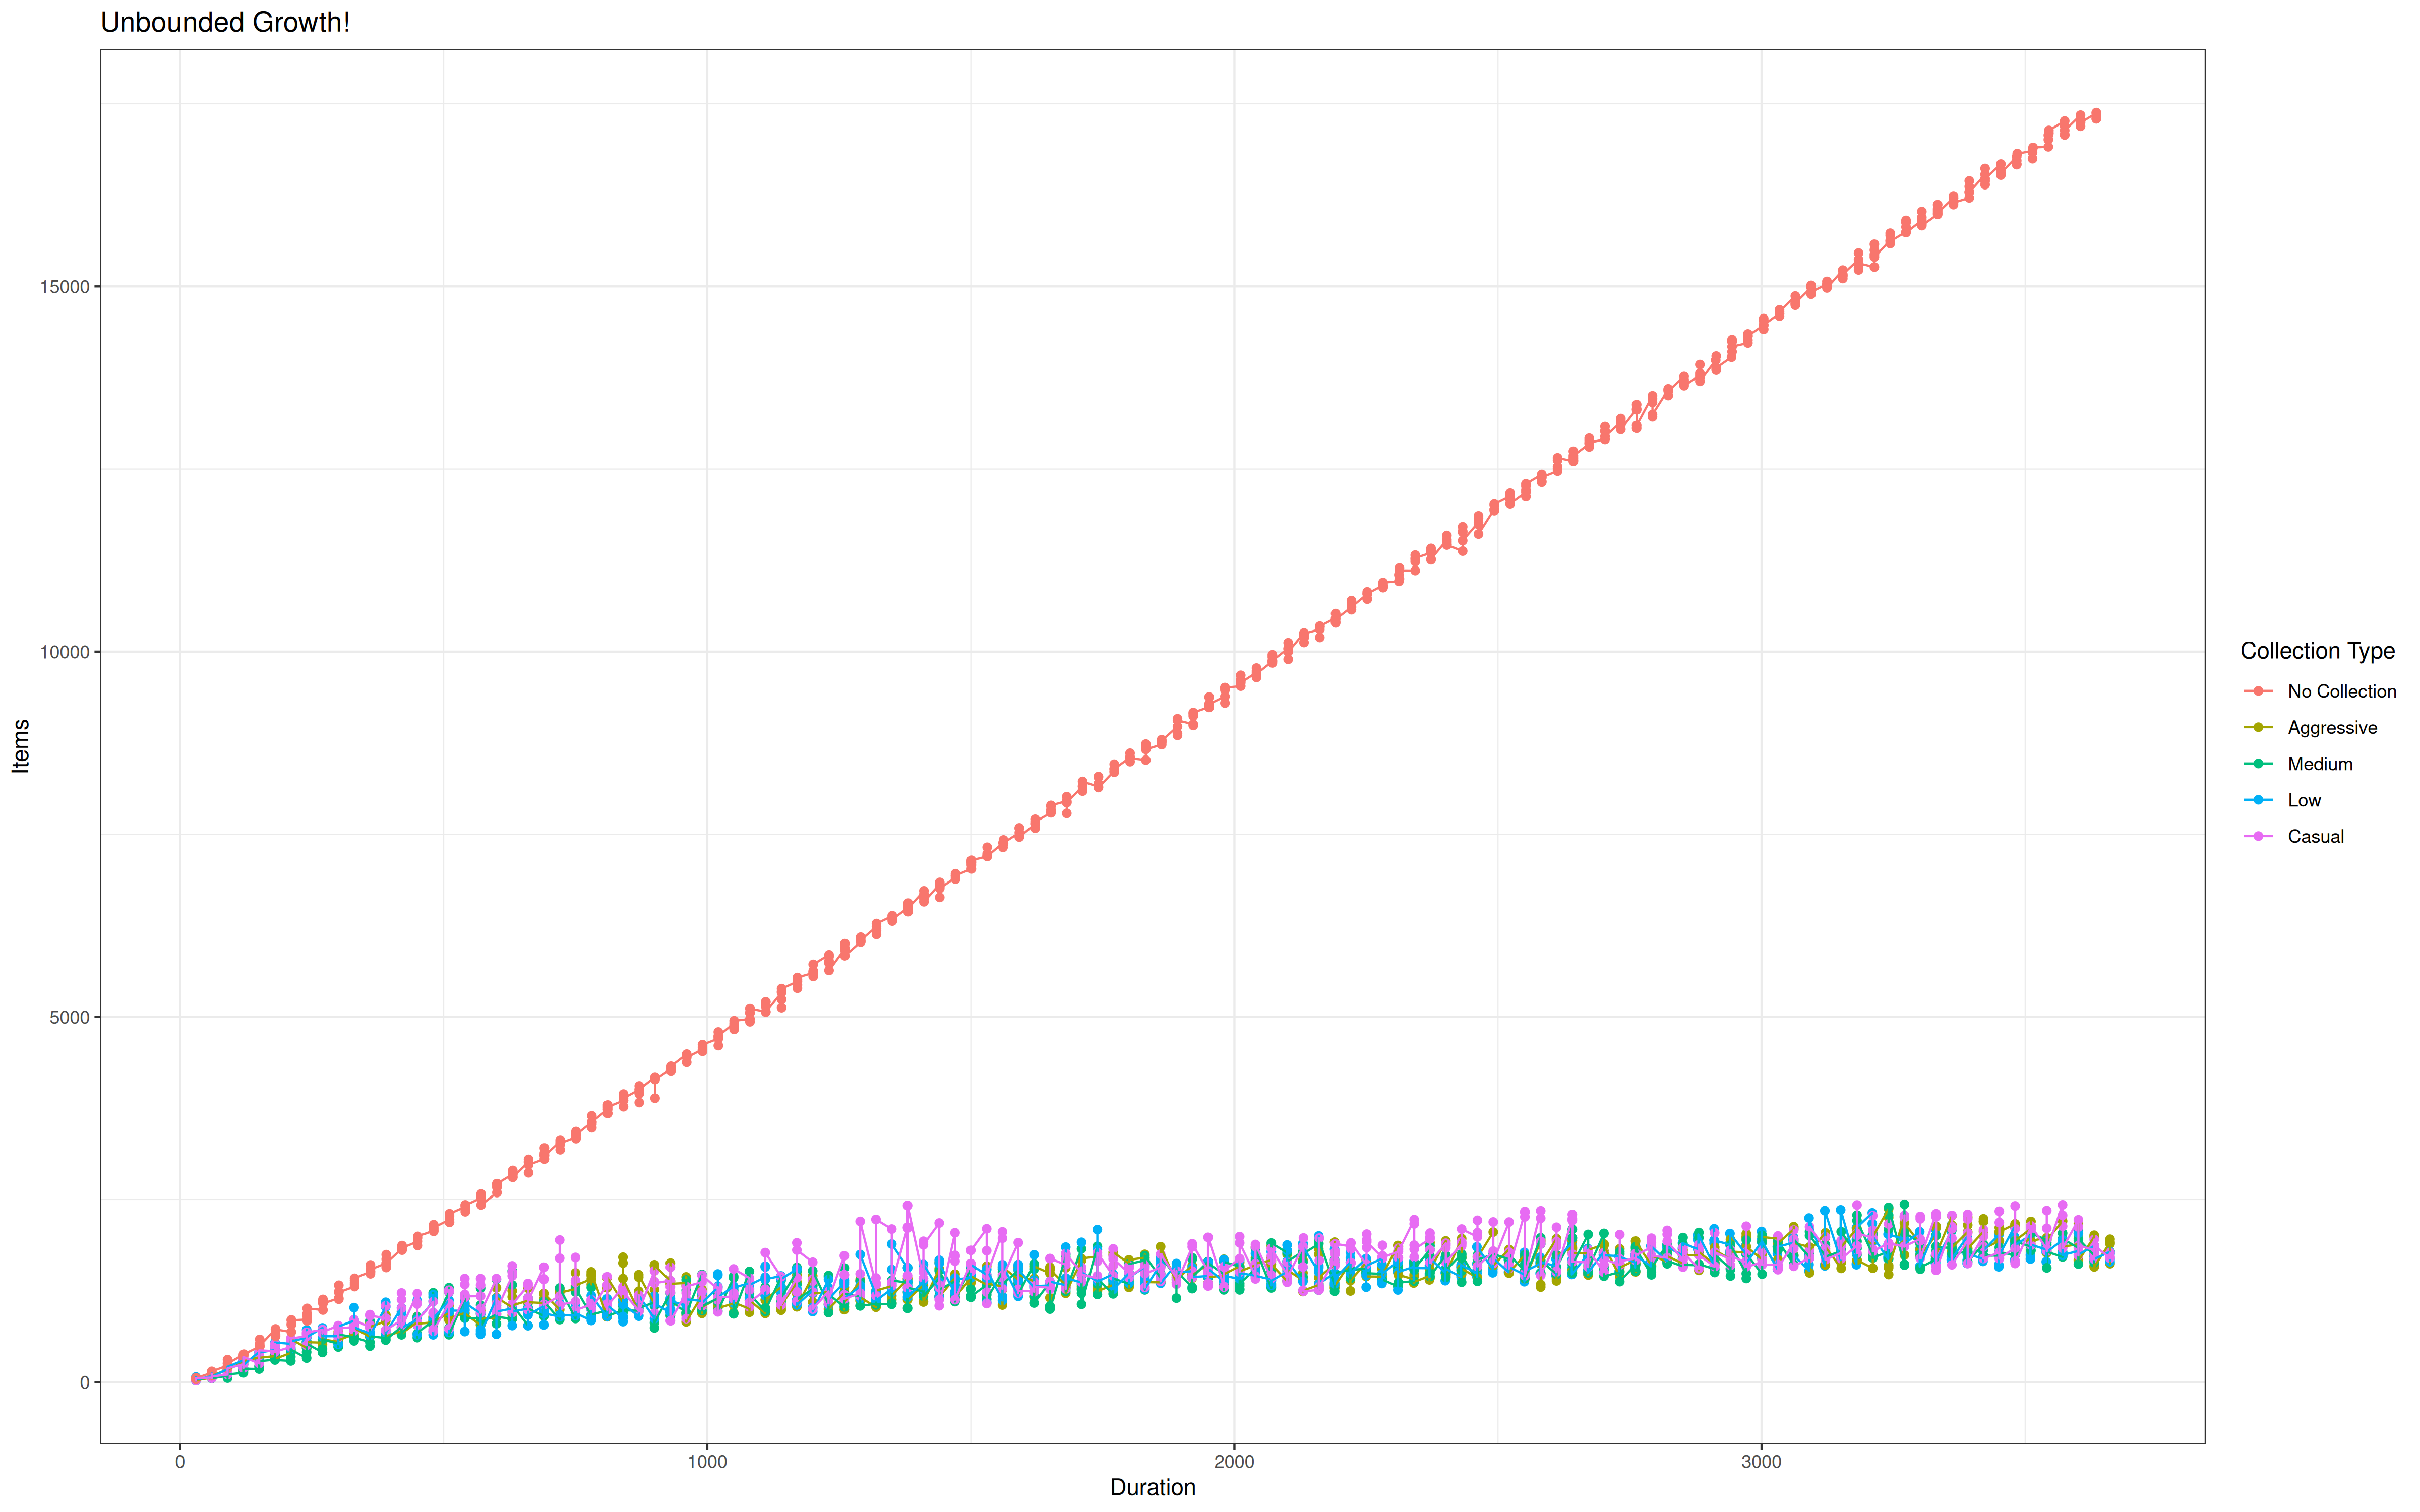
\includegraphics[width=\textwidth]{Unbounded}
    \end{frame}

    \begin{frame}
        \frametitle{Types of Collection}

        \textbf{Casual Collection}
        \begin{enumerate}
            \item \textbf{- Requires local operational ordering and bounded
                system size.}
            \item \textbf{- Implies stability.}
        \end{enumerate}

        Eager Collection
        \begin{enumerate}
            \item - Requires local operational ordering and bounded
                system size
            \item - Tracks and pushes stability information
        \end{enumerate}
    \end{frame}

    % Casual Collection
    \begin{frame}
        \includegraphics[page=2,width=\textwidth]{CRDTAnimation}
    \end{frame}
    \begin{frame}
        \includegraphics[page=3,width=\textwidth]{CRDTAnimation}
    \end{frame}
    \begin{frame}
        \includegraphics[page=4,width=\textwidth]{CRDTAnimation}
    \end{frame}
    \begin{frame}
        \includegraphics[page=5,width=\textwidth]{CRDTAnimation}
    \end{frame}
    \begin{frame}
        \includegraphics[page=6,width=\textwidth]{CRDTAnimation}
    \end{frame}
    \begin{frame}
        \includegraphics[page=7,width=\textwidth]{CRDTAnimation}
    \end{frame}
    \begin{frame}
        \includegraphics[page=8,width=\textwidth]{CRDTAnimation}
    \end{frame}
    \begin{frame}
        \includegraphics[page=9,width=\textwidth]{CRDTAnimation}
    \end{frame}
    \begin{frame}
        \includegraphics[page=10,width=\textwidth]{CRDTAnimation}
    \end{frame}
    \begin{frame}
        \includegraphics[page=11,width=\textwidth]{CRDTAnimation}
    \end{frame}
    \begin{frame}
        \includegraphics[page=12,width=\textwidth]{CRDTAnimation}
    \end{frame}
    \begin{frame}
        \includegraphics[page=13,width=\textwidth]{CRDTAnimation}
    \end{frame}
    \begin{frame}
        \includegraphics[page=14,width=\textwidth]{CRDTAnimation}
    \end{frame}
    \begin{frame}
        \includegraphics[page=15,width=\textwidth]{CRDTAnimation}
    \end{frame}
    \begin{frame}
        \includegraphics[page=16,width=\textwidth]{CRDTAnimation}
    \end{frame}
    \begin{frame}
        \includegraphics[page=17,width=\textwidth]{CRDTAnimation}
    \end{frame}
    \begin{frame}
        \includegraphics[page=18,width=\textwidth]{CRDTAnimation}
    \end{frame}
    \begin{frame}
        \includegraphics[page=19,width=\textwidth]{CRDTAnimation}
    \end{frame}
    \begin{frame}
        \includegraphics[page=20,width=\textwidth]{CRDTAnimation}
    \end{frame}

    \begin{frame}
        \frametitle{Types of Collection}
        Casual Collection
        \begin{enumerate}
            \item - Requires local operational ordering and bounded
                system size
            \item - Implies stability.
        \end{enumerate}

        \textbf{Eager Collection}
        \begin{enumerate}
            \item \textbf{- Requires local operational ordering and bounded
                system size.}
            \item \textbf{- Tracks and pushes stability information.}
        \end{enumerate}
    \end{frame}

    % Eager Collection
    \begin{frame}
        \includegraphics[page=21,width=\textwidth]{CRDTAnimation}
    \end{frame}
    \begin{frame}
        \includegraphics[page=22,width=\textwidth]{CRDTAnimation}
    \end{frame}
    \begin{frame}
        \includegraphics[page=23,width=\textwidth]{CRDTAnimation}
    \end{frame}
    \begin{frame}
        \includegraphics[page=24,width=\textwidth]{CRDTAnimation}
    \end{frame}
    \begin{frame}
        \includegraphics[page=25,width=\textwidth]{CRDTAnimation}
    \end{frame}
    \begin{frame}
        \includegraphics[page=26,width=\textwidth]{CRDTAnimation}
    \end{frame}
    \begin{frame}
        \includegraphics[page=27,width=\textwidth]{CRDTAnimation}
    \end{frame}
    \begin{frame}
        \includegraphics[page=28,width=\textwidth]{CRDTAnimation}
    \end{frame}
    \begin{frame}
        \includegraphics[page=29,width=\textwidth]{CRDTAnimation}
    \end{frame}
    \begin{frame}
        \includegraphics[page=30,width=\textwidth]{CRDTAnimation}
    \end{frame}
    \begin{frame}
        \includegraphics[page=31,width=\textwidth]{CRDTAnimation}
    \end{frame}

    \begin{frame}[shrink]
        \frametitle{Primary Objective}
        \begin{center}
        \begin{minipage}{4in}
         To measure the memory reduction of using garbage collection in
         combination with an OR-Set while keeping the properties of a
         Conflict-free Replicated Data Type. Limited to 1.5 person
         weeks over 12 weeks.
        \end{minipage}
        \end{center}
    \end{frame}

    \begin{frame}
        \frametitle{Solution Description}
        The ORSet Research Database

        \begin{enumerate}
        \item Written in C.
        \item Communicates using RPCs.
        \item Implements Casual Collection \& Eager Collection.
        \item Configurable (1) merge rate, (2) system size, and (3) eager
            collection rate.
        \end{enumerate}
    \end{frame}

    \begin{frame}[shrink]
        \frametitle{Hypothesis}
        \begin{center}
        \begin{minipage}{4in}
        1. While the data size of a node not using garbage collection
        will grow linearly with the amount of operations; using garbage
        collection will bound growth to the data growth rate.

        \bigskip

        2. An increase in garbage collection rate will lead to a
        decrease in total items at a given time.
        \end{minipage}
        \end{center}
    \end{frame}

    \begin{frame}[shrink]
        \frametitle{Goal Tree}
        \begin{center}
            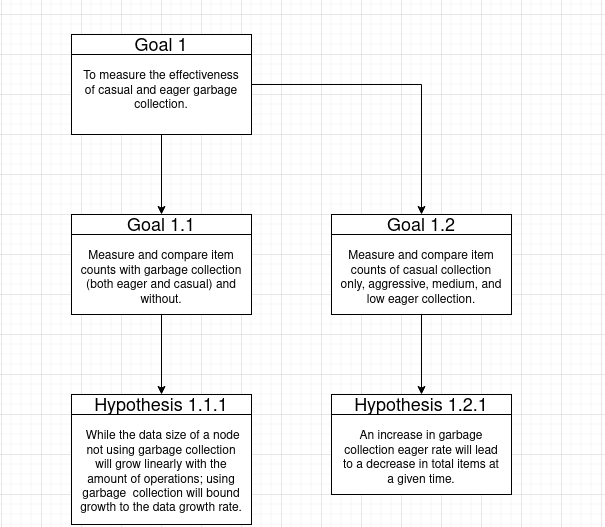
\includegraphics[width=0.8\textwidth]{GoalTree}
        \end{center}
    \end{frame}

    % Results bounded growth
    % Show unbounded with lines and slopes

    \begin{frame}
        \frametitle{Bounded Growth}
        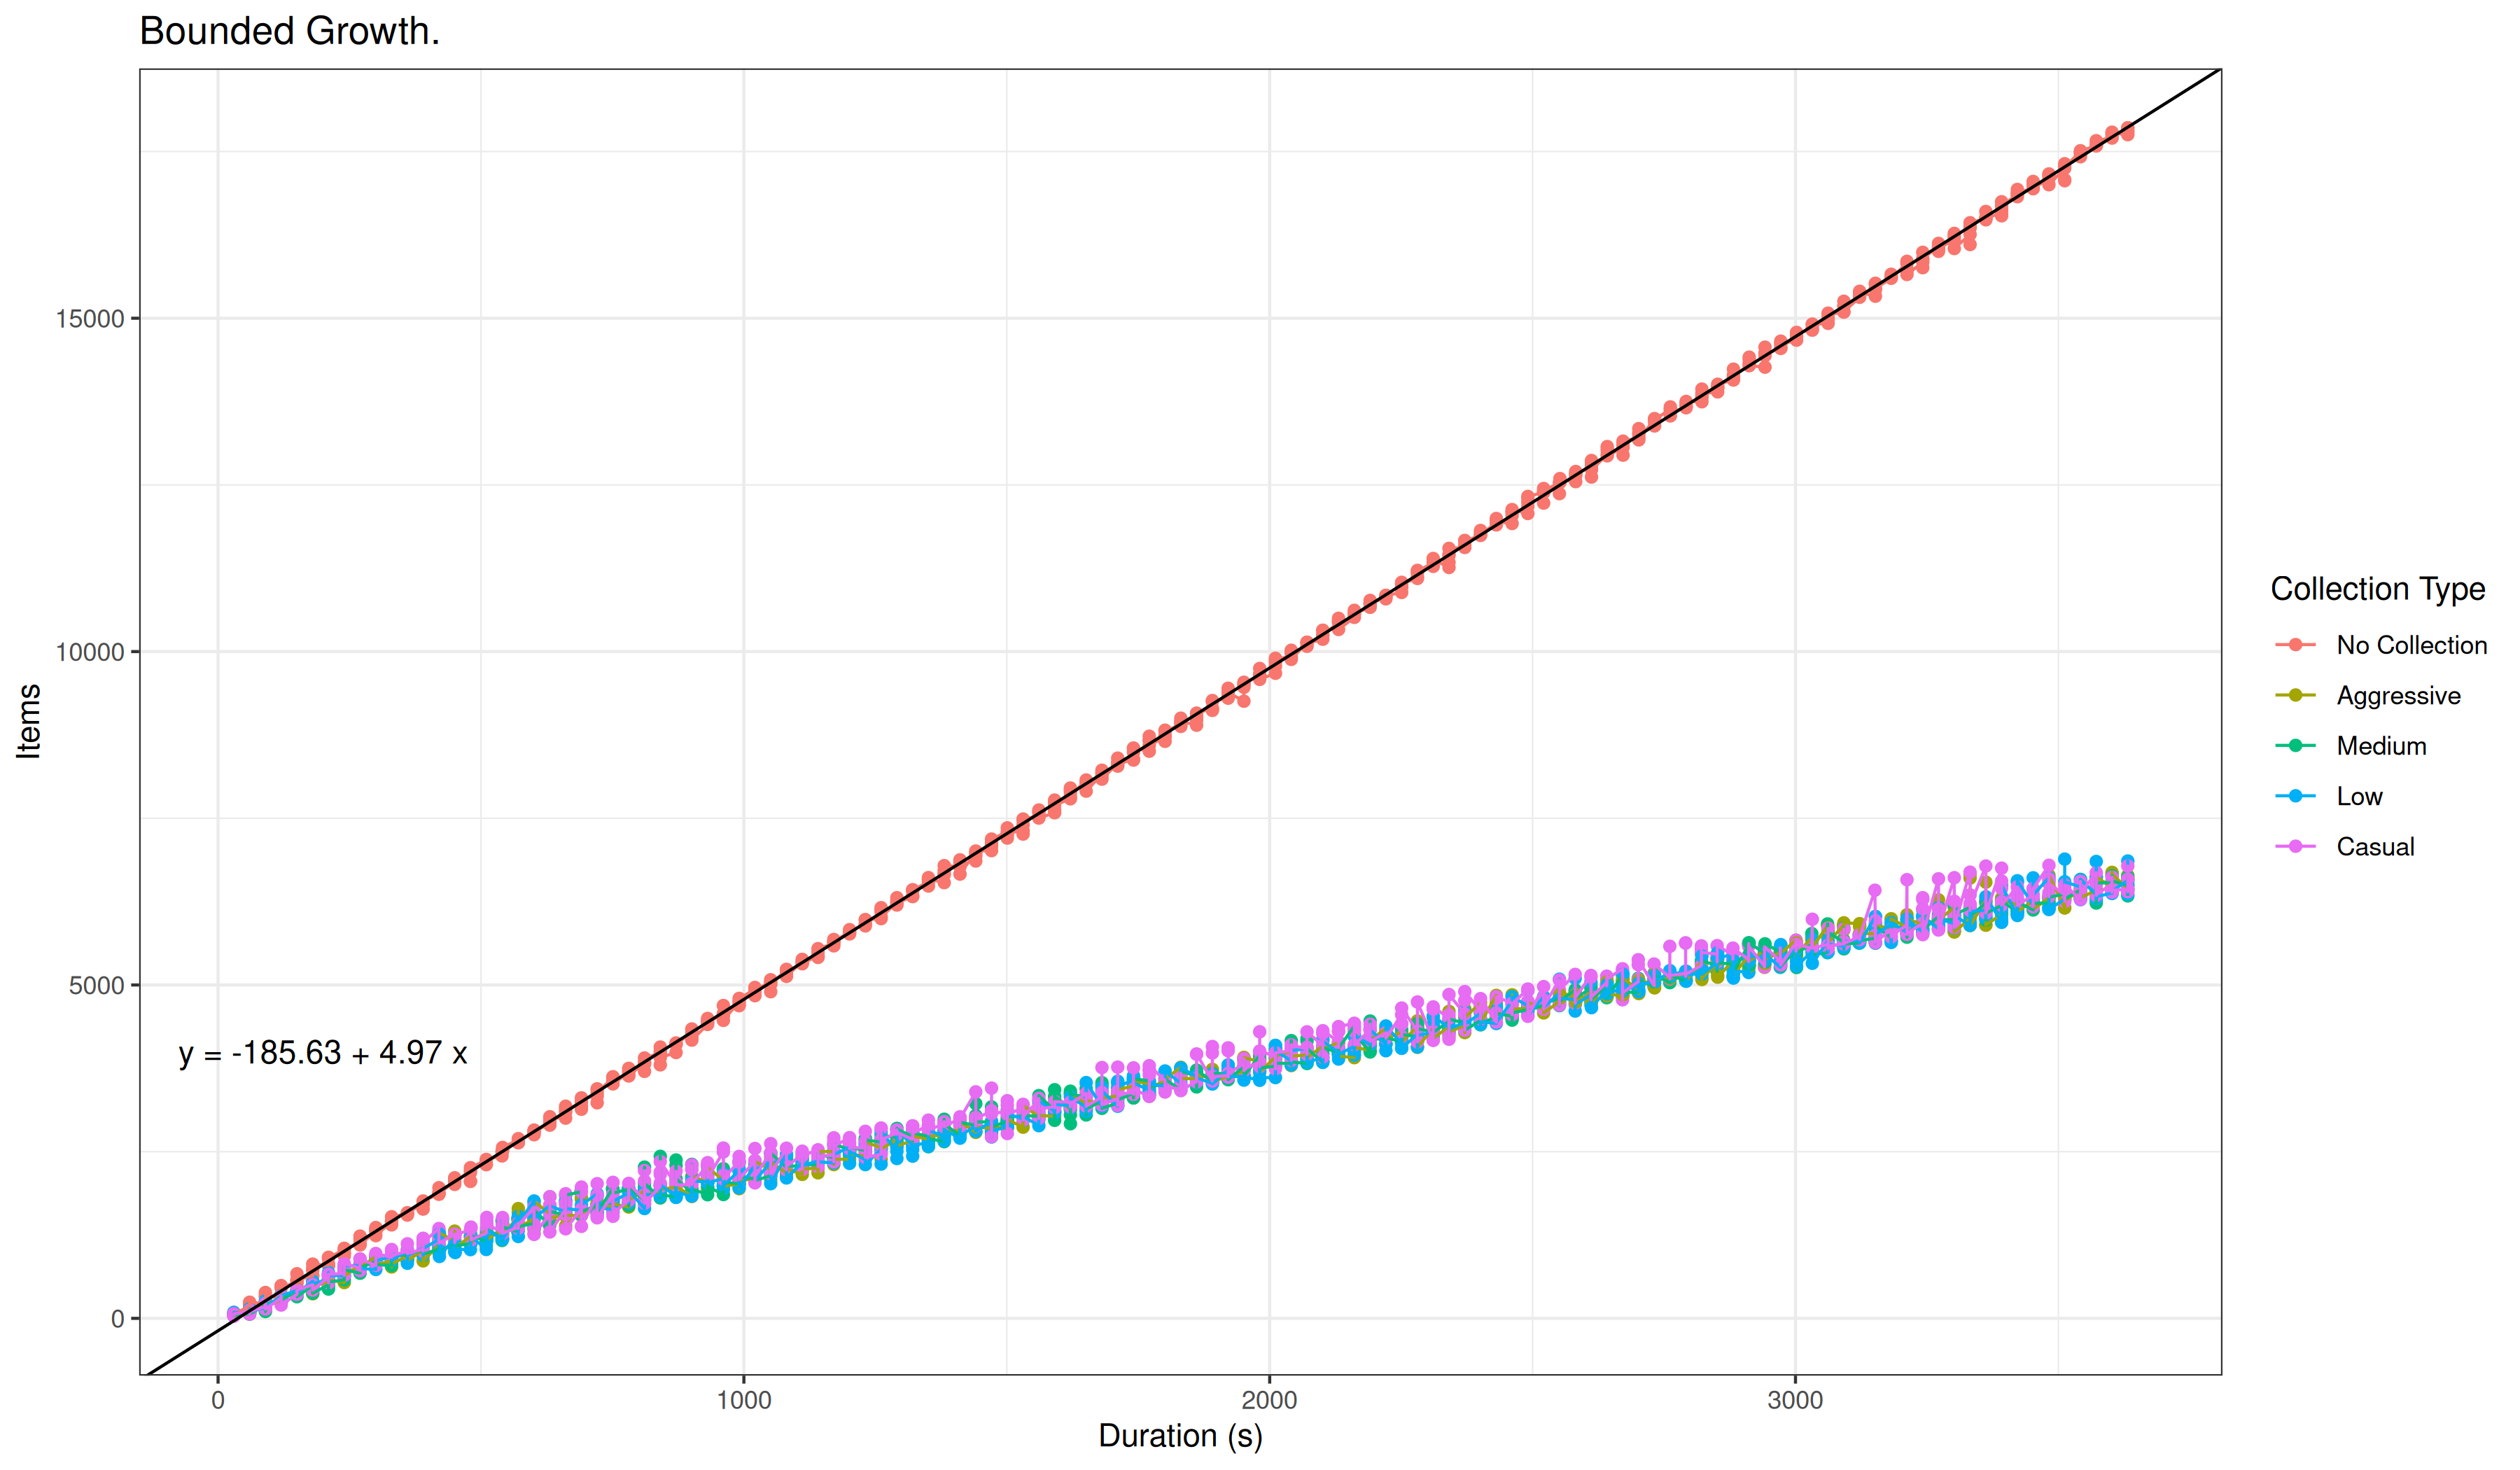
\includegraphics[width=\textwidth]{BoundedGrowth1_2}
    \end{frame}


    \begin{frame}
        \frametitle{Bounded Growth}
        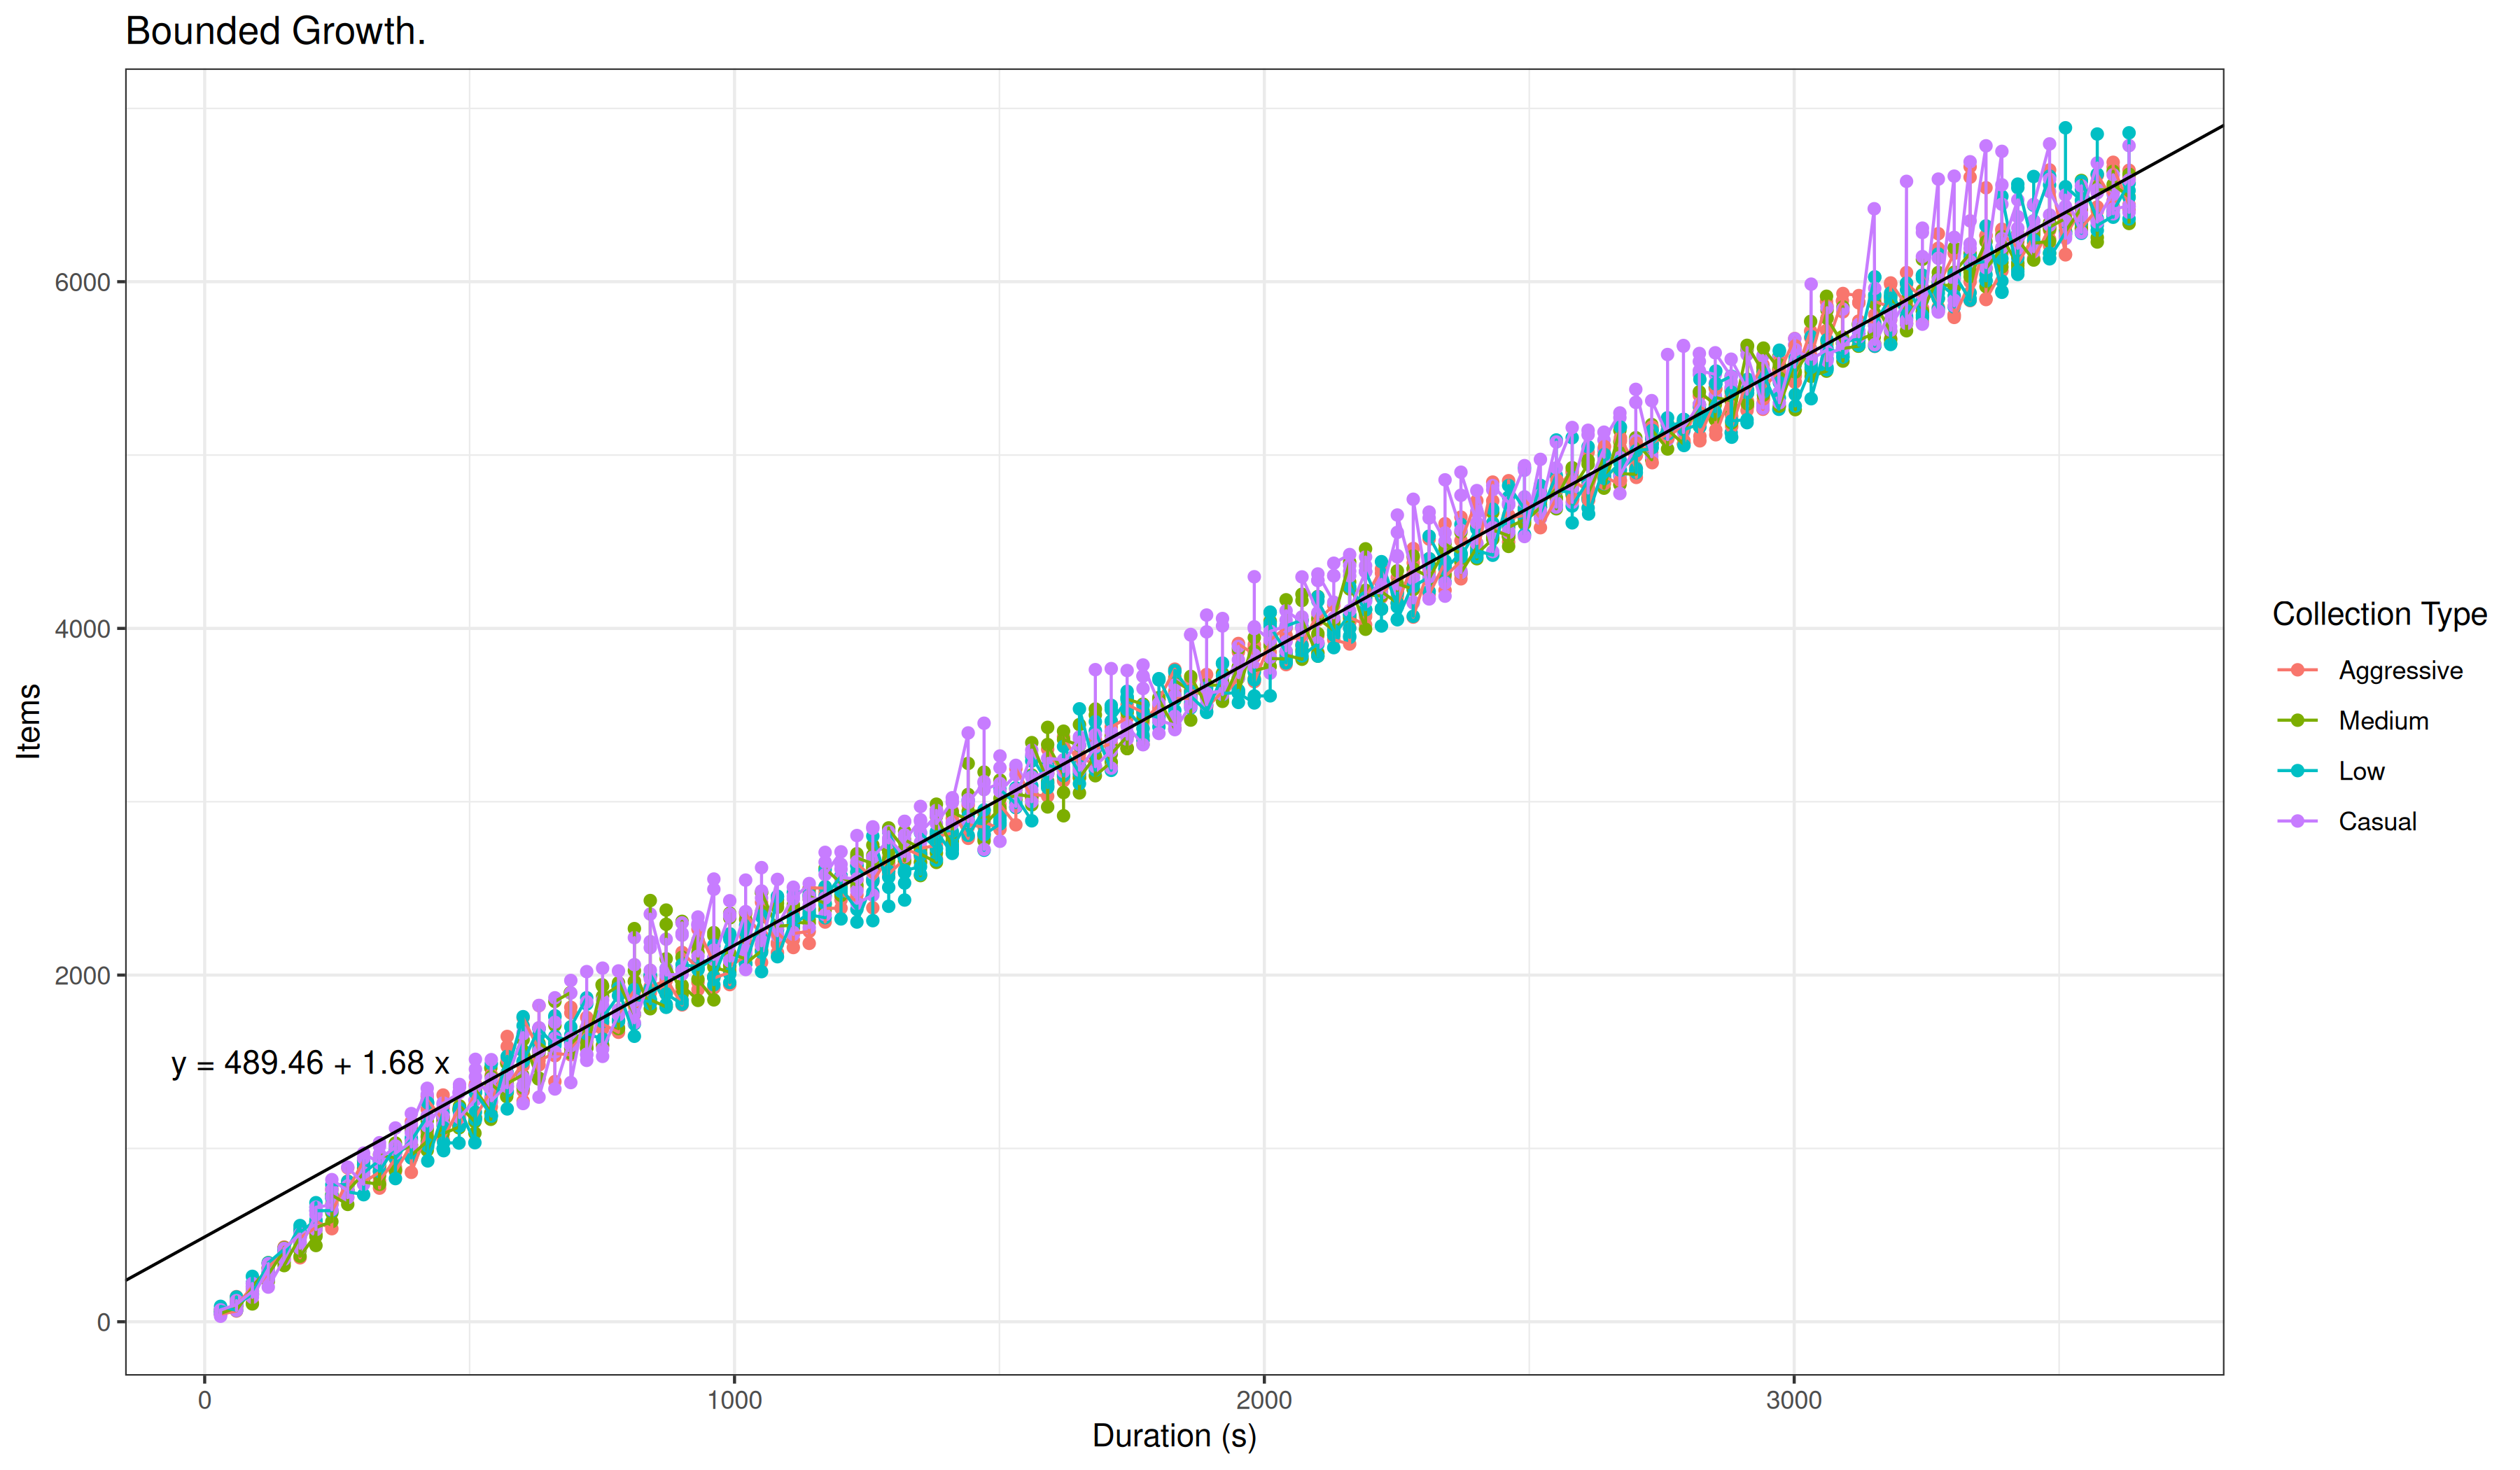
\includegraphics[width=\textwidth]{BoundedGrowth2_2}
    \end{frame}

    \begin{frame}[shrink]
        \frametitle{Bounded Growth}

        Linear regression:

        {\tiny X=$(1000, 3600)$}

        \begin{center}
            $Items = 489.5 + 1.683 Duration$
        \end{center}

        \begin{center}
            \begin{tabular}{ ||c c||}
                \hline
                Setting & Value \\
                \hline
                Growth Rate & $1/3$ \\
                Nodes & 5 \\
                Operation Rate & 1s \\
                Merge Rate & 30s \\
                Eager Rate & Varies \\
                \hline
            \end{tabular}
        \end{center}

        \begin{center}
            $5Nodes*1/3 Items Per Sec = 1.66 Items Per Sec$
            $5Nodes*1 Operation Per Sec = 5 Operations Per Sec$
        \end{center}
    \end{frame}

    \begin{frame}
        \frametitle{Collection Types}
        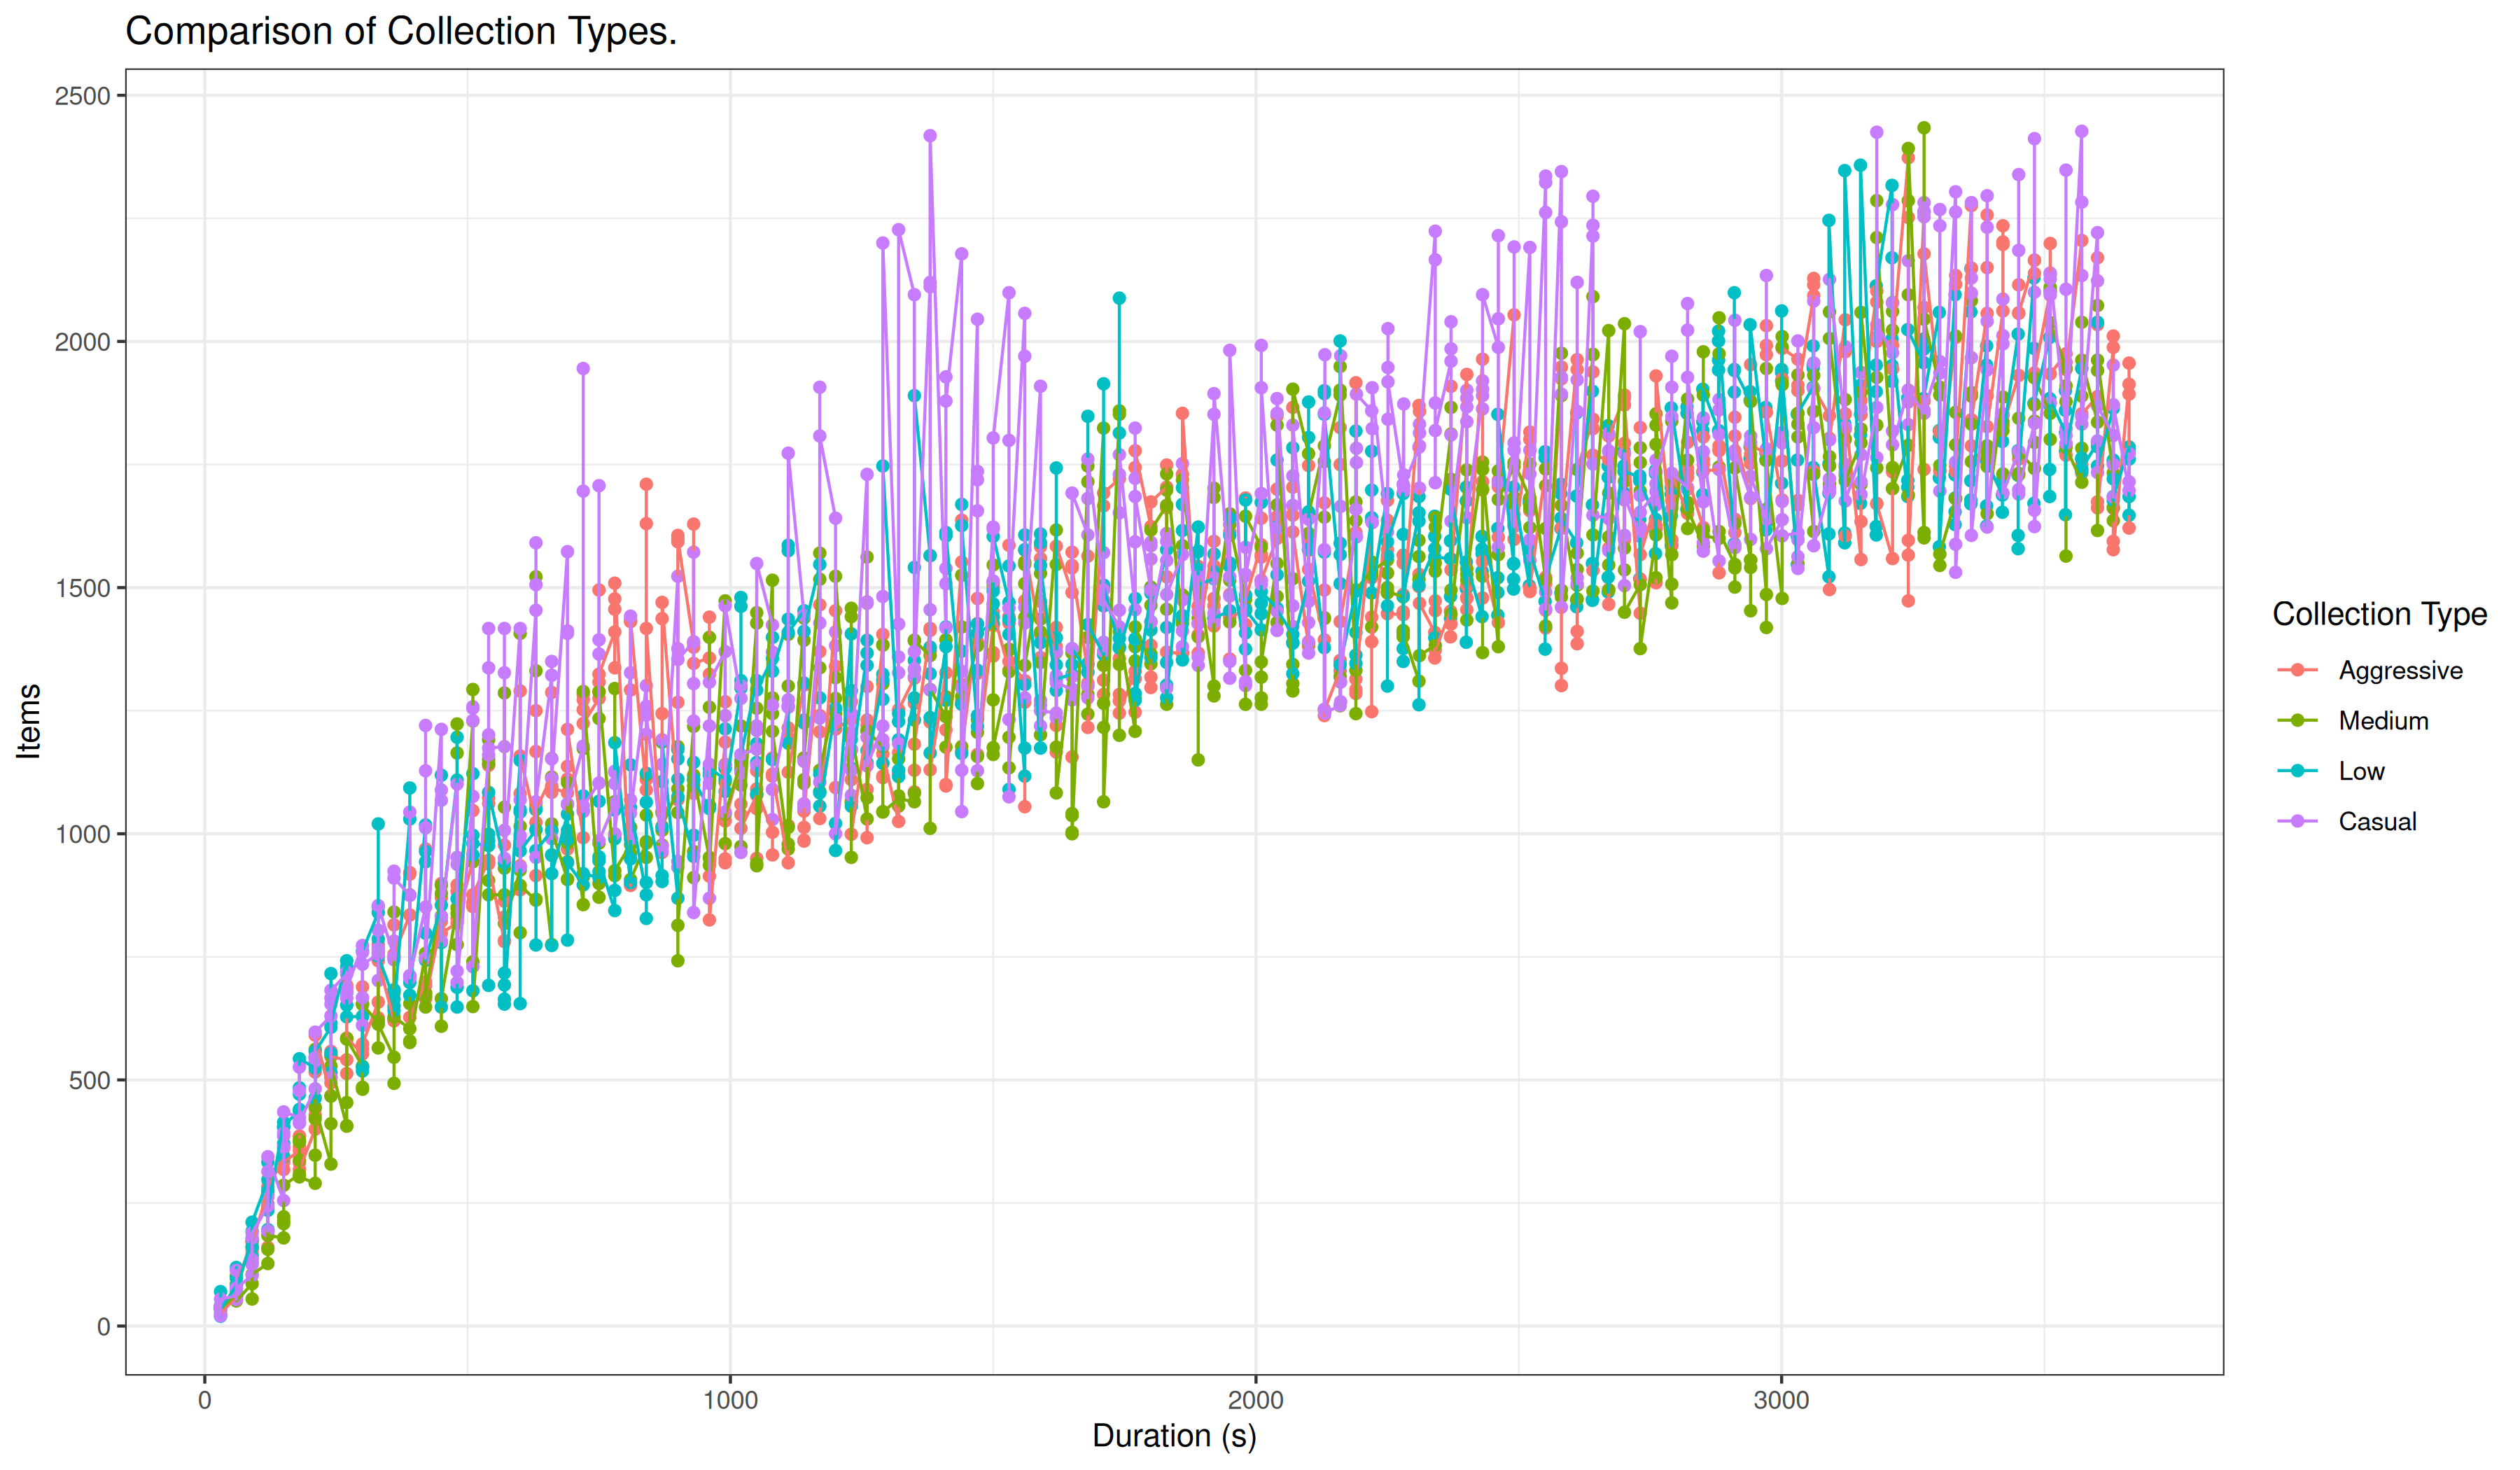
\includegraphics[width=\textwidth]{CollectionType1_1}
    \end{frame}
    \begin{frame}
        \frametitle{Collection Types}
        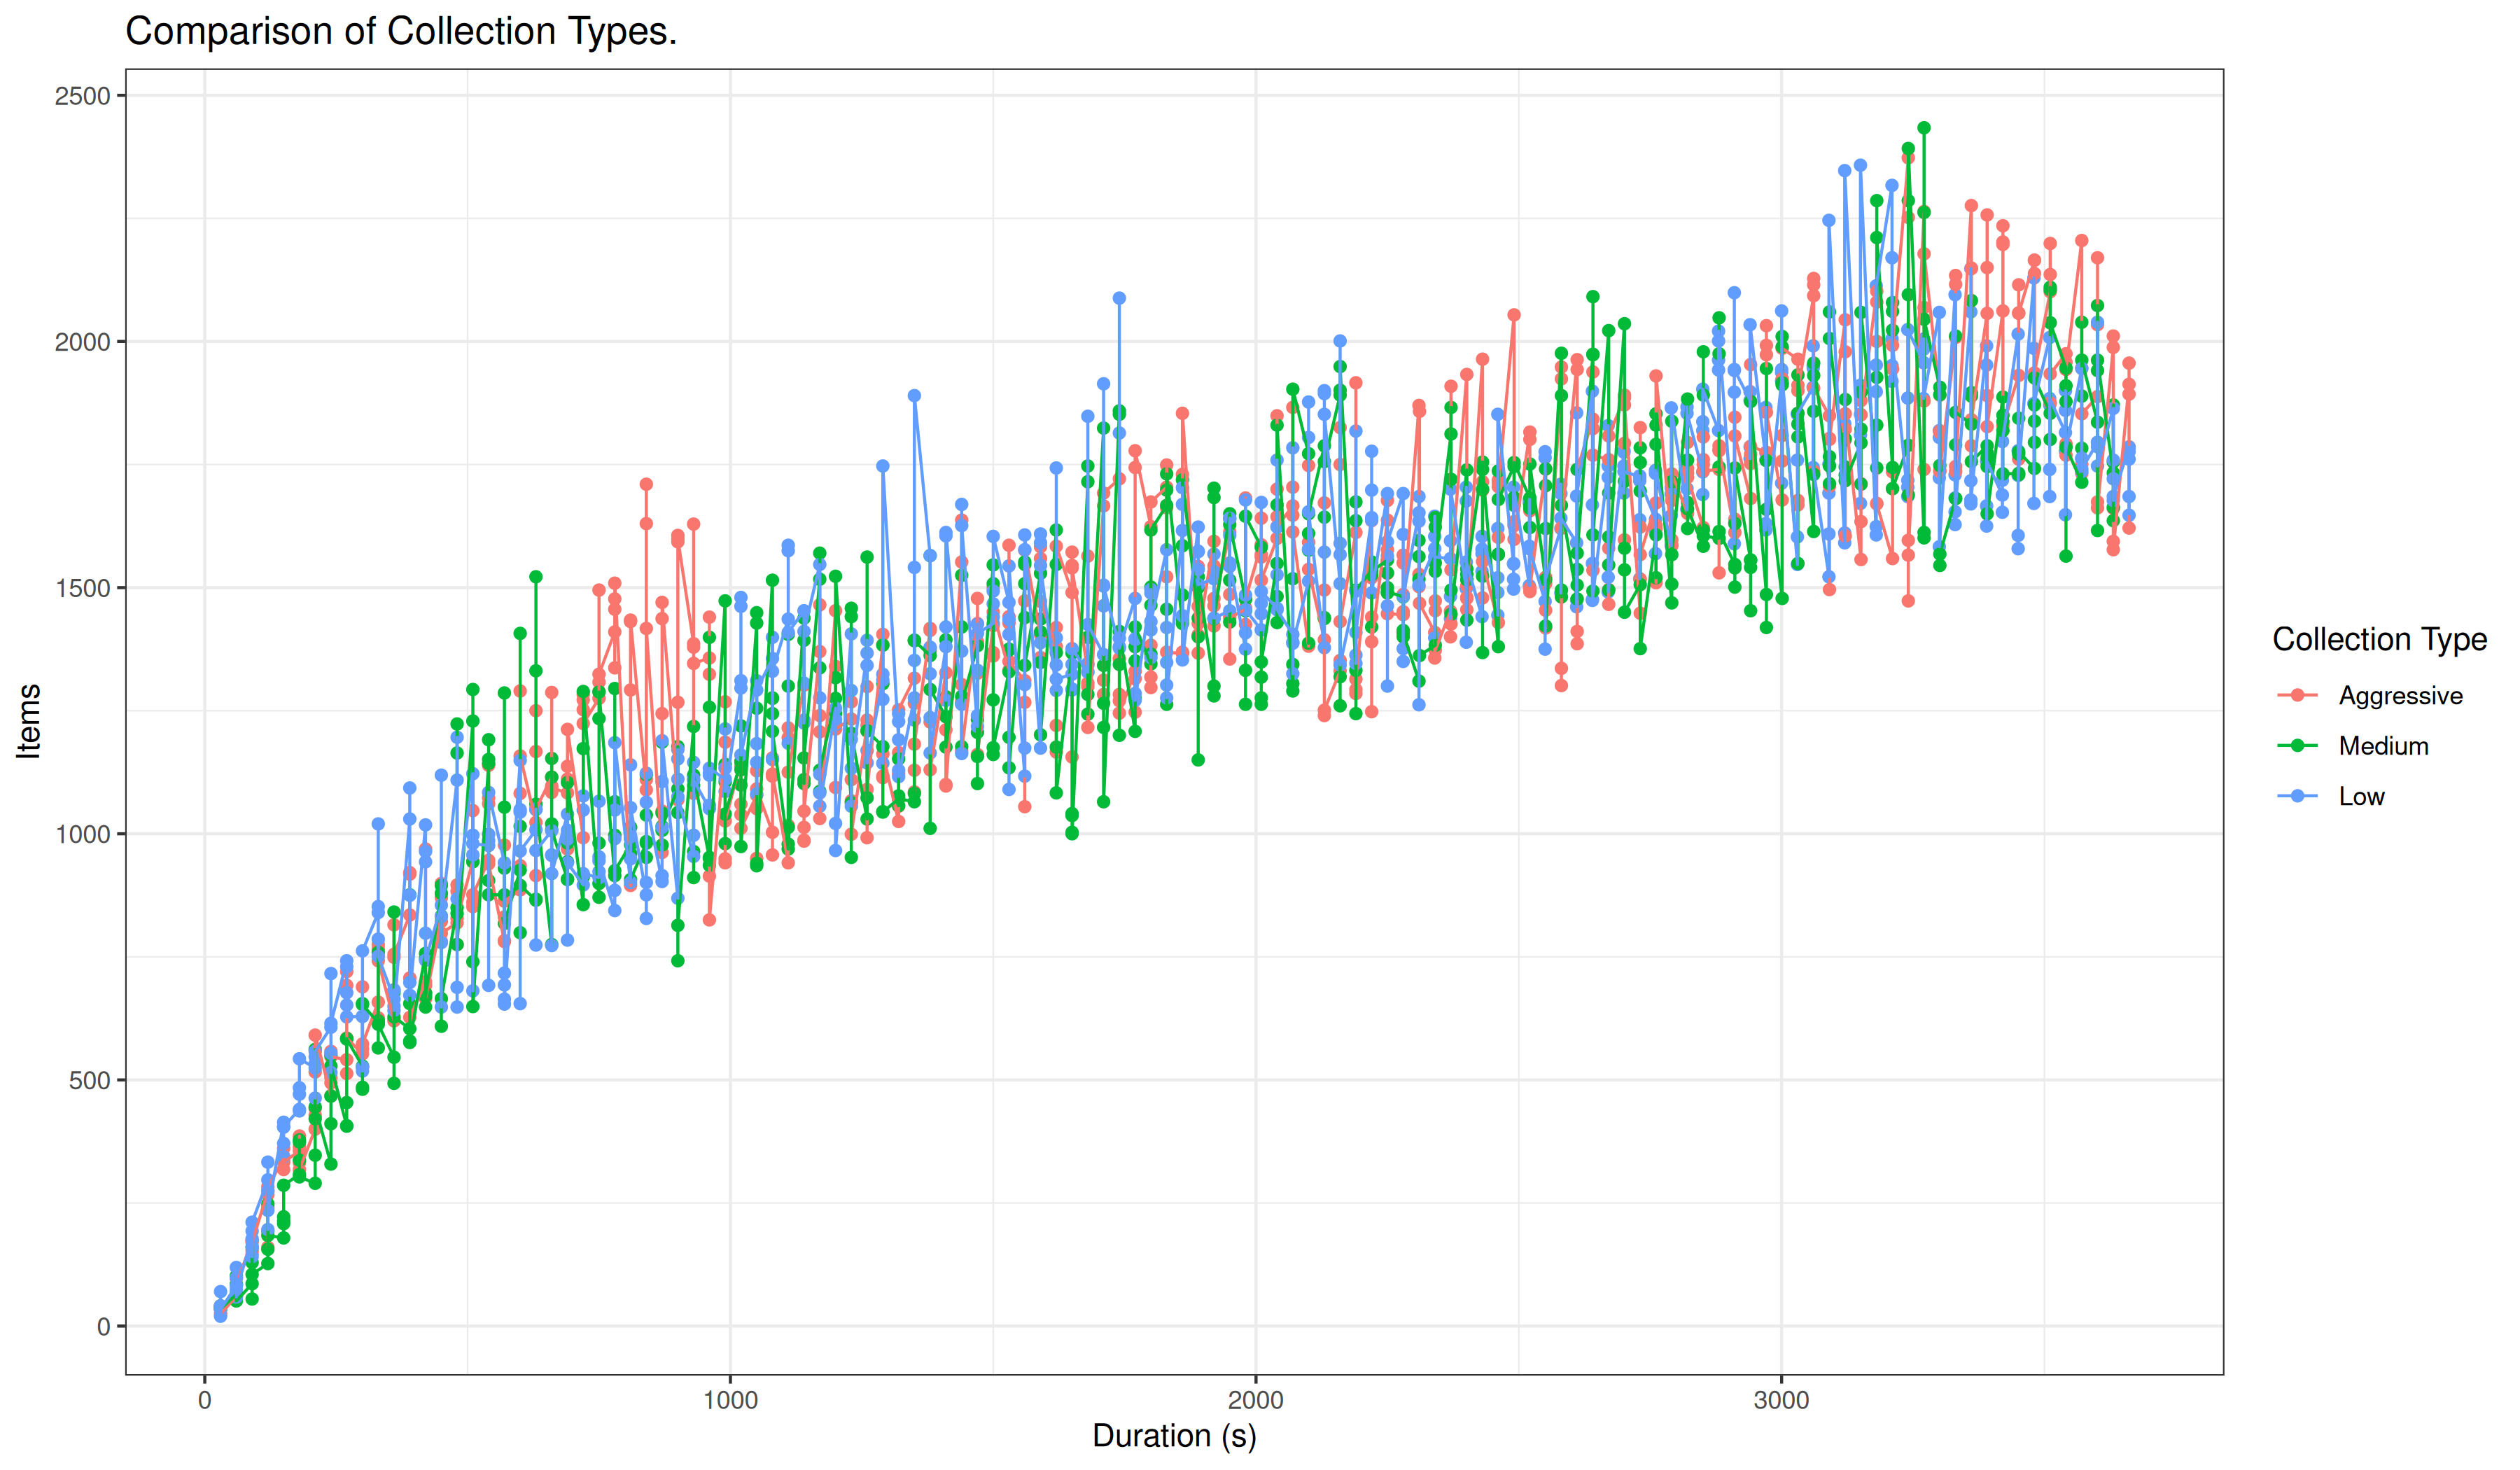
\includegraphics[width=\textwidth]{CollectionType2_1}
    \end{frame}

    \begin{frame}
        \frametitle{Collection Types}
        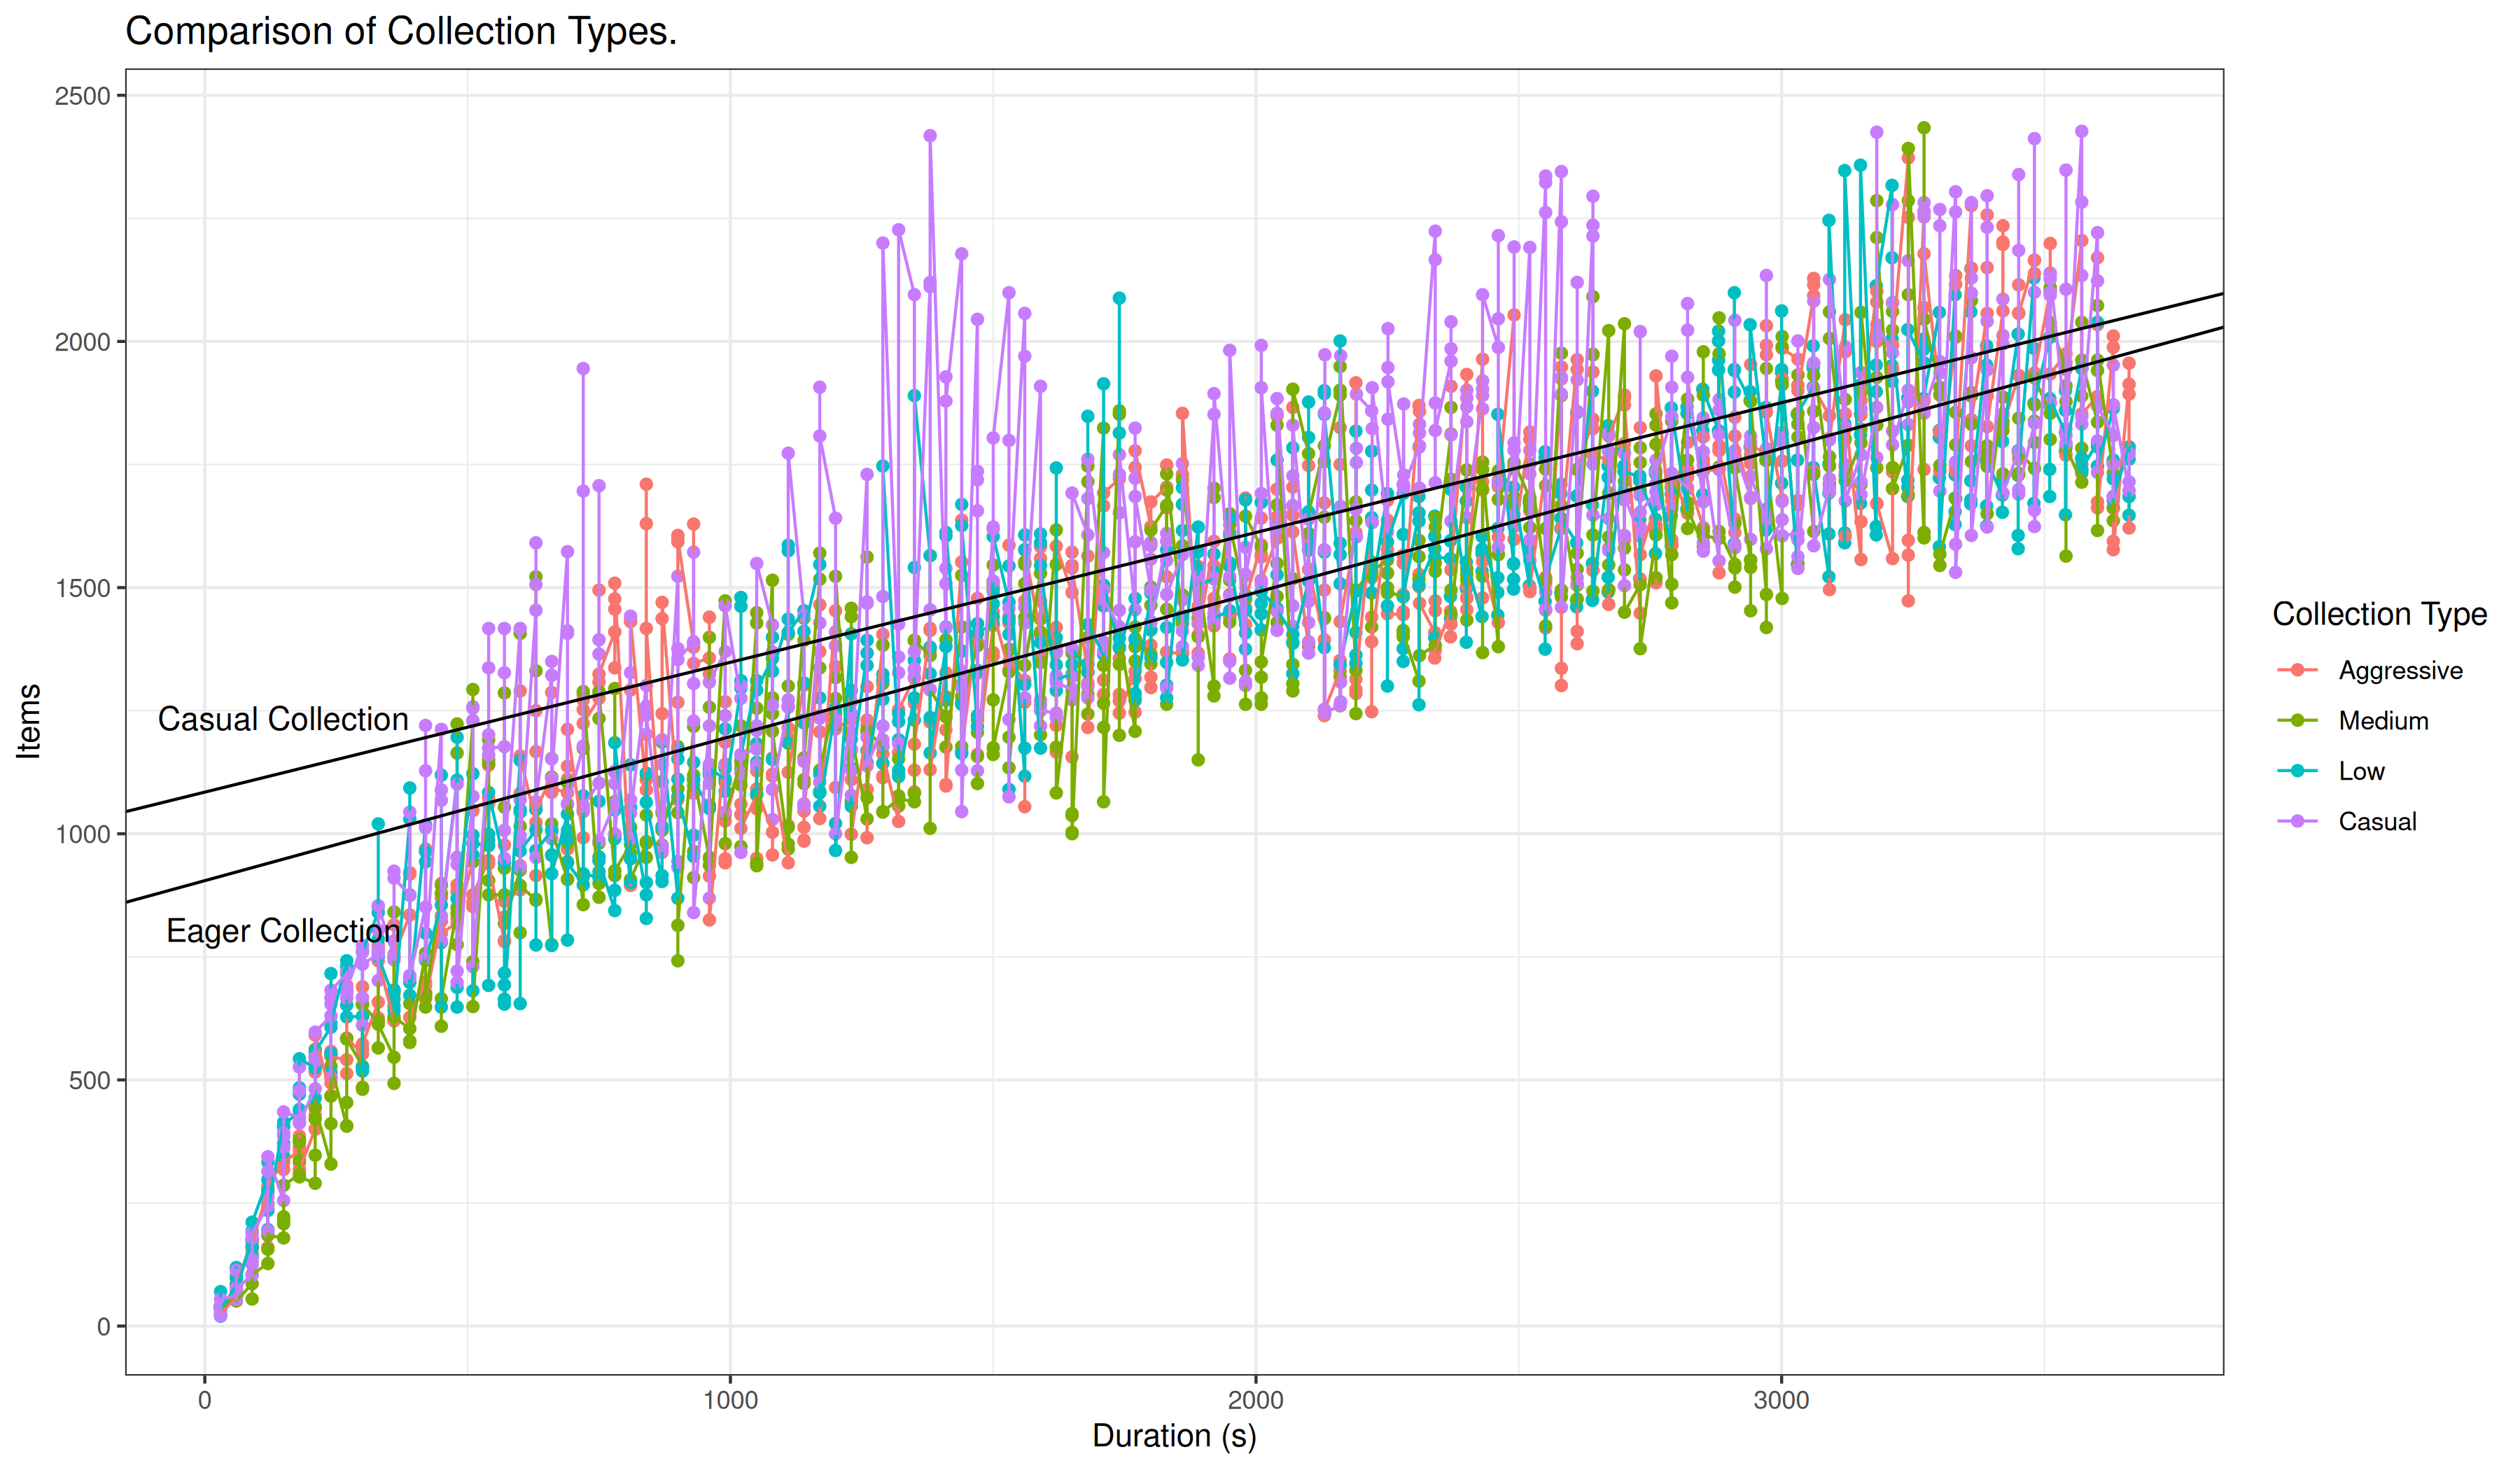
\includegraphics[width=\textwidth]{CollectionType3_1}
    \end{frame}

    \begin{frame}[shrink]
        \frametitle{Collection Types}
        Does eager collection make a difference?

        \bigskip
        \bigskip
        \bigskip

        \begin{center}
            At X = 1000...

            Eager Collection = 2,148.724

            Casual Collection = 2,242.656

            Difference: $\sim$94 tombstones

            $\sim$4.4\%

        \end{center}
    \end{frame}

    \begin{frame}
        \frametitle{Collection Types}
        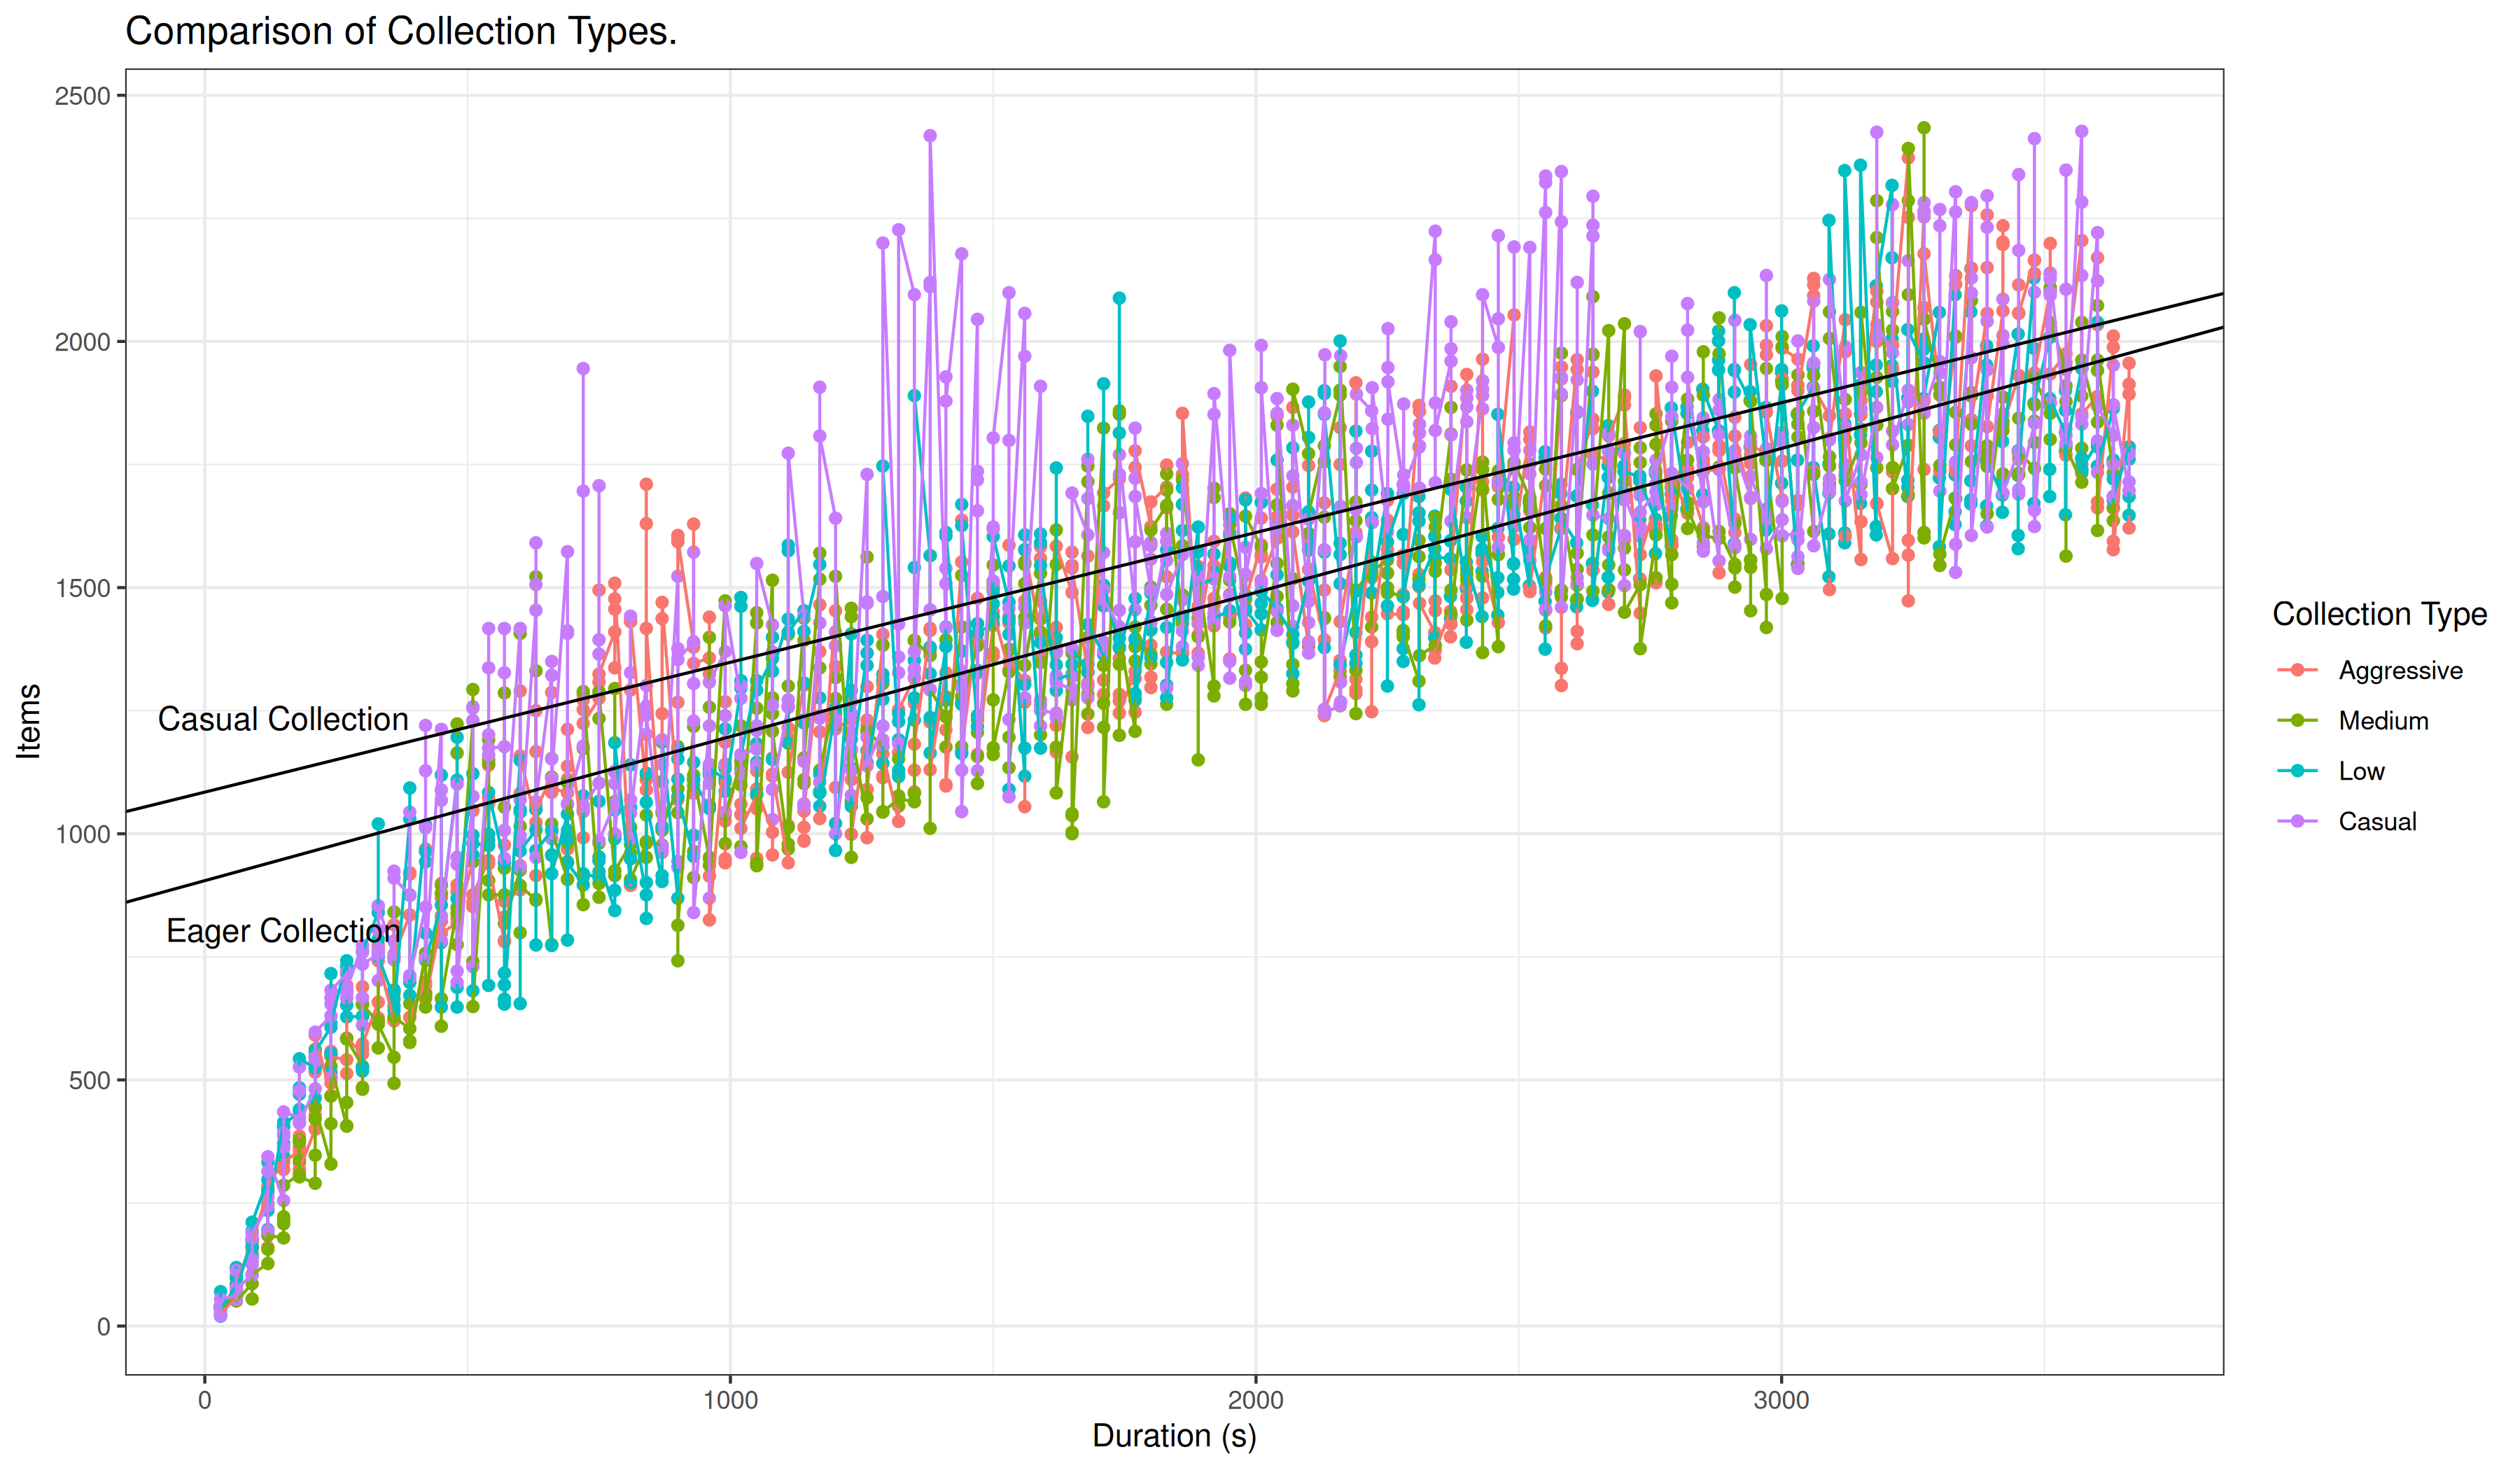
\includegraphics[width=\textwidth]{CollectionType3_1}
    \end{frame}

    \begin{frame}[shrink]
        \frametitle{Collection Types}
        Are the slopes different?

        \bigskip
        \bigskip
        \bigskip

        \begin{center}
            Hypothesis Test:

            {\small $H_{0}: \beta_{1a} - \beta_{1b} = 0$}

            \pause

            \textbf{p-value = 0.0449}
        \end{center}
    \end{frame}

    \begin{frame}
        \frametitle{Conclusion}

        \begin{center}
        \begin{minipage}{4in}
        \begin{enumerate}
            \item 1. The growth rate of an OrSet using either garbage
                collection algorithm is based on growth rate of
                the data as opposed to the operation rate.
            \bigskip
            \item 2. The difference between casual collection and eager
                collection can be seen through a shrinking difference in
                items over time.
        \end{enumerate}
        \end{minipage}
        \end{center}

    \end{frame}

    % Future research
    \begin{frame}
        \frametitle{Future Research}

        \begin{center}
        \begin{minipage}{4in}
        \begin{enumerate}
            \item Test which eager collection rate are best when
                balanced with network overhead.
            \bigskip
            \item Explore why the gap between casual collection and eager
                collection closes over time.
            \bigskip
            \item Prove and verify an OrSet network joining model that
                is compatibile with both eager and casual collection.
            \bigskip
            \item Measure garbage collection performance in a clustered
                network topology.
        \end{enumerate}
        \end{minipage}
        \end{center}
    \end{frame}

    \begin{frame}
        \includegraphics[page=21,width=\textwidth]{original}
    \end{frame}

\end{document}
